\section{Mechanization and Countermodels}
\label{sec:mechanization}

\statusestablished

Gate 7 adds two complementary verification layers. I use a finite-model oracle for concrete countermodels and bounded exhaustive searches, and Lean for general semantic theorems that must not depend on a finite bound. Gate 8 extends the same discipline to comparative variants, modal-frame minimization, and the Fitting intension/extension reconstruction. This separation prevents the absence of a small countermodel from being mistaken for a proof and, conversely, allows an apparently successful proof interface to be tested for semantic vacuity.

\subsection{Finite-model regression layer}
\label{sec:finite-layer}

The executable checker implements the four information values, involutive FDE negation, finite accessibility relations, actualist existence, four-valued property extensions and positivity, signed necessary entailment, support-based Godlikeness, positive essence, and the Gate-6 regularity conditions.

The regression suite machine-checks both two-world T2 countermodels from Gate 6. The glut model satisfies the encoded Gate-5 control stack and \(COMP_P^G\) but violates \(CONS_G^G\), while the gap model satisfies the same control stack and \(CONS_G^G\) but violates \(COMP_P^G\). Both refute \(T2^+\).

The checker also validates the Gate-5 obstruction to unrestricted positive T1. A one-world reflexive model with no actual entities and glutty positivity for a property and its complement satisfies strong A1 and \(A2^+\), while positive support for the property does not yield positive possible actual exemplification. This is the executable counterpart of the distinction between mere positive support and truth-only positivity.

A first bounded search retains 204 models satisfying the original small control antecedent and verifies \(T2^+\) in every retained model. A broader exhaustive two-world, one-entity \(G,Z\) family then varies positivity of \(Z\) and its complement independently while fixing FDE complement exemplification and full bilateral \(G\)-support semantics. The family also fixes the Scott-control positivity of Godlikeness itself, taking \(P(G)=\True\) and \(P(\neg G)=\False\) at both worlds; the search is therefore exhaustive relative to an A3-style positivity of \(G\) rather than over all positivity assignments. In this broader family, 873 models satisfy
\[
 A1_L,\qquad R^+,\qquad COMP_P^G,\qquad CONS_G^G,
\]
and every one of them satisfies \(T2^+\). Dropping any one of these four assumptions while retaining the other three produces a \(T2^+\) countermodel within the same bounded family. I therefore treat this as bounded individual indispensability, not global model-theoretic minimality.

The same oracle now exports selected witnesses as directed Kripke graphs. Figure~\ref{fig:gate7-a1l-countermodel} shows the first countermodel isolated after dropping only \(A1_L\): \(R^+\), \(COMP_P^G\), and \(CONS_G^G\) remain true while \(T2^+\) fails. The two HTML-style node tables display the complete local FDE matrix. Each row records its value in \(\{\True,\False,\Both,\Neither\}\) together with the underlying positive and negative support bits. The four arrows are read directly from the model's complete two-world accessibility relation.

\begin{figure}[htbp]
  \centering
  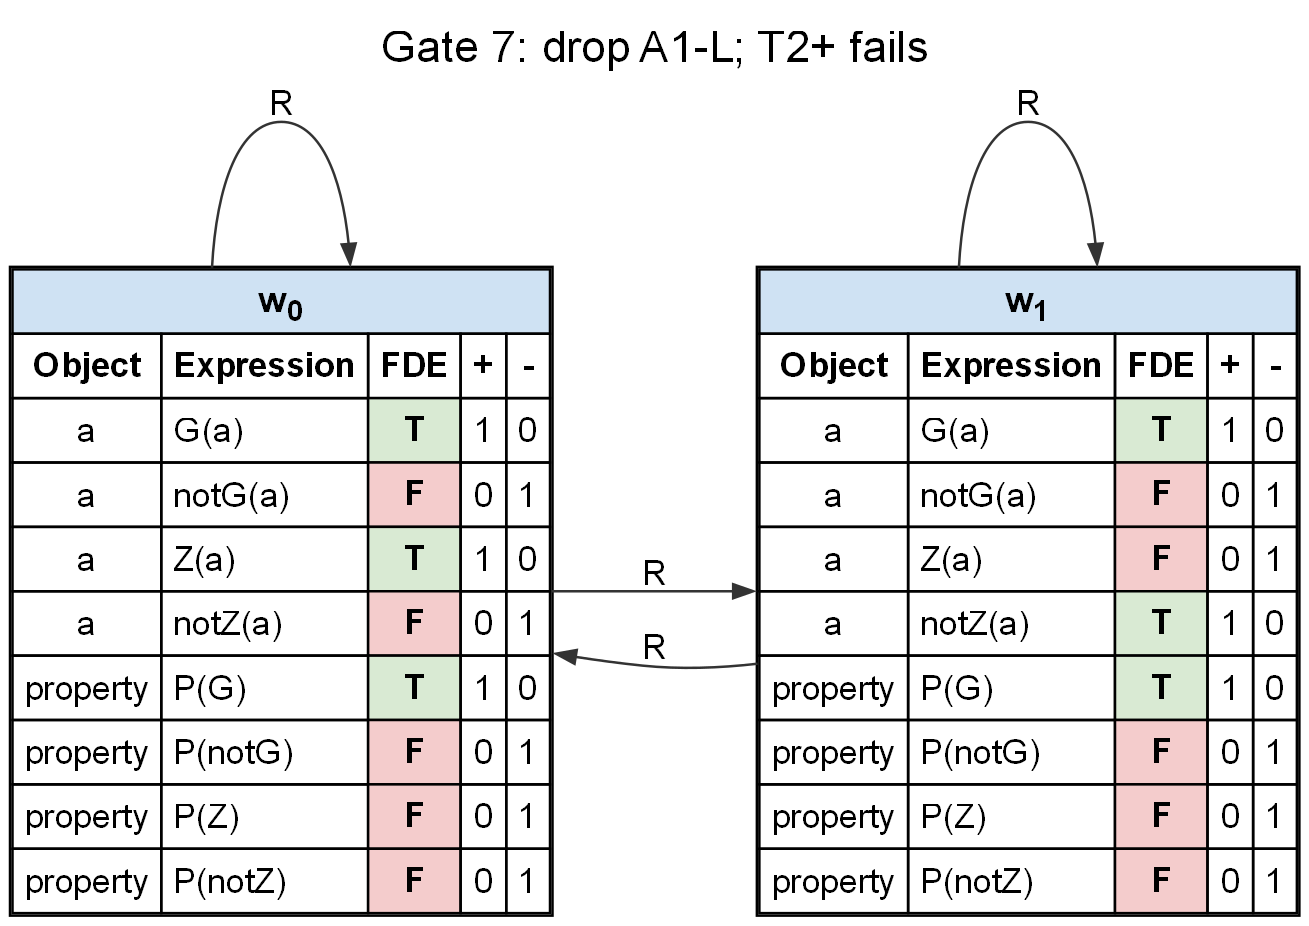
\includegraphics[width=0.96\linewidth]{figures/gate7_drop_a1_l_countermodel.png}
  \caption{The first Gate-7 \(T2^+\) countermodel found when only \(A1_L\) is dropped. The graph is generated by \texttt{formal/finite/visualize\_gate7\_models.py} from the same matrix family used in the 873-model exhaustive regression.}
  \label{fig:gate7-a1l-countermodel}
\end{figure}

The checker also verifies the schema-level equivalence
\[
  \MCp\leftrightarrow\MCm
\]
on a negation-closed two-world test family. The equivalence concerns schemata closed under substitution by negation, not a pointwise identity for one isolated formula valuation.

Gate 8 adds comparative witnesses. The support/exact comparison confirms that both Gate-6 T2 countermodels are support-Godlike but fail project-internal exact positive Godlikeness, while a separate exact-Godlike fixture still permits genuine \(\Both\) gluts. A complete-S5 bilateral Anderson fixture has positive necessary Godlike existence while a contingent formula application refutes positive modal collapse. Separate Scott and Anderson S4-style two-world models are reflexive and transitive but not symmetric and refute the corresponding reduced T3 conclusions.

The Fitting branch adds two further finite witnesses. First, a three-world two-entity model uses a selected negation-closed extensional property domain and satisfies the admissible Fitting recovery stack. At the root world the current frozen \(G\)-extension is both possibly and necessarily actually exemplified de re, and de-dicto Godlikeness is possible, but de-dicto necessary Godlikeness fails because the extension of \(G\) changes at another accessible world. The model therefore separates the two readings when the explicit extension-stability condition introduced below is absent.

Second, a complete two-world S5 model satisfies the encoded admissible Fitting stack, extension stability, and positive necessary actual Godlikeness. Its selected extension domain nevertheless contains genuine inconsistent information: one admissible extension takes value \(\Both\) on an entity, together with its FDE negation. A separate contingent intension \(Q\) satisfies
\[
  \pos{Q(a)}@w_0
\]
but not
\[
  \pos{\Box Q(a)}@w_0.
\]
Thus the present admissible bilateral Fitting candidate has an explicit necessary-God / no-positive-collapse model. This is a finite countermodel to collapse for the candidate, not an unbounded theorem about every Fitting semantics.

\subsection{Lean layer}
\label{sec:lean-layer}

The Lean package is pinned to Lean 4.30.0. It formalizes the four-valued carrier, FDE negation, conjunction and disjunction, bilateral relational modality, bilateral actualist quantification, signed necessary entailment, support-based Godlikeness, bilateral essence, and necessary-existence interfaces.

Lean proves the collapse-channel theorem generally at schema level and the Gate-5 truth-only possibility theorem
\[
  A1_R+A2^+\Longrightarrow T1_T.
\]
The principal Gate-6 Scott recovery theorem is machine-checked without a finite bound:
\[
  NegExemplification
  +G\text{-sup}
  +A1_L
  +R^+
  +REG_G
  \Longrightarrow T2^+.
\]

Gate 8 sharpens the later modal dependency. Once Scott \(T2^+\) is available, Lean proves
\[
  \operatorname{Sym}(R)
  +PossibleGod
  +T2^+
  +A5^+
  +NE\text{-sup}
  +G\text{-sup}
  \Longrightarrow T3^+.
\]
Reflexivity and transitivity are absent. Reflexivity enters only in the separate implication \(T3^+\Rightarrow GW\) and in the current essence-compressed collapse theorem
\[
  \operatorname{Refl}(R)
  +T2^+
  +T3^+
  +G\text{-sup}
  +CONST
  \Longrightarrow\MCp.
\]

For project-internal exact positive Godlikeness, Lean proves
\[
  G\text{-exact}^+\Rightarrow G\text{-sup}^+
\]
and
\[
  G\text{-exact}^+ + R^+\Longrightarrow T2_{\mathrm{exact}}^+.
\]
For Anderson, the literature-grounded positive interfaces and project-specific bilateral negative evidence are mechanized separately. Under classical coherence the negative necessary-exemplification, Godlikeness, essence, necessary-actual-exemplification, and necessary-existence clauses recover the complements of their positive counterparts. The positive Anderson necessary-existence branch reduces to symmetry alone:
\[
\begin{split}
  &\operatorname{Sym}(R)
  +PossibleG_A
  +G_A\text{-realization}
  +P^+(G_A)
  +A2^+\\
  &\qquad
  +NE_A\text{-realization}
  +P^+(NE_A)
  \Longrightarrow T3_A^+.
\end{split}
\]

\subsection{Classical recovery and verification discipline}
\label{sec:verification-discipline}

The Scott, Anderson, and admissible Fitting branches each have explicit recovery interfaces rather than relying on an informal assertion that the bilateral semantics ``becomes classical.'' Exact higher-order correspondence with the complete AFP/HOL developments is nevertheless a separate publication audit item.

The repository treats a countermodel or an obstruction theorem as a result rather than as a failed proof attempt. The unrestricted Fitting-comprehension obstruction is a particularly useful example: a theorem initially looked stronger because it lacked \(R^+\), but mechanization plus domain analysis revealed that the unrestricted regularity package excluded its intended witnesses. The admissible-domain reconstruction makes the subsequent theorem non-vacuous and is independently checked by finite models.

The explicit actualist quotient adds a third consistency check between the abstract and bounded layers. Lean's \texttt{FittingActualistQuotient.lean} constructs quotient entities, proves bilateral extension push/pull round trips, characterizes existence factorization, and identifies quotient entailment with ordinary entailment on pullbacks. The matching finite fixture exhausts all sixteen bilateral extensions in a two-entity one-class model and compares all 256 ordered entailment pairs. It also checks that \(\Both\) and \(\Neither\) survive quotienting and that split actual existence blocks representative-independent quotient interpretation.

The filter follow-up is split in the same way. The Lean quotient-filter module proves abstractly that point evaluation is a prime truth-order delta-filter which designates \(\Both\) but is not complement-deciding because of \(\Neither\). The finite oracle enumerates all filter families on the sixteen-element two-point quotient algebra and separately checks the non-adjunctive two-filter condition and a non-vacuous \(COMP\)-failure fixture.

The deferred paired-neighborhood layer now has the same two-sided validation. Lean proves modal duality, exact relational representation, and complement-dual classical recovery for arbitrary world types. The finite regression exhausts all \(256\) local two-world pairs of neighborhood families and all \(1024\) relational operator comparisons. The complete Python regression suite currently contains 31 tests.

All executable and Lean sources are maintained under \texttt{formal/}, with CI configured to run both tracks. General claims are promoted to machine-checked status only after an unbounded Lean theorem is present, while finite witnesses are reported as finite witnesses with their model bounds explicit. Appendix~\ref{sec:correspondence} maps every claim of the form ``Lean proves \(\dots\)'' in this manuscript to the named declaration that discharges it, and every bounded count to the fixture that produces it. Where the text abbreviates a premise list as a ``stack'', the Lean signature listed there is the authoritative statement.
